% Options for packages loaded elsewhere
\PassOptionsToPackage{unicode}{hyperref}
\PassOptionsToPackage{hyphens}{url}
\PassOptionsToPackage{dvipsnames,svgnames,x11names}{xcolor}
%
\documentclass[
  letterpaper,
  DIV=11,
  numbers=noendperiod,
  oneside]{scrartcl}

\usepackage{amsmath,amssymb}
\usepackage{lmodern}
\usepackage{iftex}
\ifPDFTeX
  \usepackage[T1]{fontenc}
  \usepackage[utf8]{inputenc}
  \usepackage{textcomp} % provide euro and other symbols
\else % if luatex or xetex
  \usepackage{unicode-math}
  \defaultfontfeatures{Scale=MatchLowercase}
  \defaultfontfeatures[\rmfamily]{Ligatures=TeX,Scale=1}
\fi
% Use upquote if available, for straight quotes in verbatim environments
\IfFileExists{upquote.sty}{\usepackage{upquote}}{}
\IfFileExists{microtype.sty}{% use microtype if available
  \usepackage[]{microtype}
  \UseMicrotypeSet[protrusion]{basicmath} % disable protrusion for tt fonts
}{}
\makeatletter
\@ifundefined{KOMAClassName}{% if non-KOMA class
  \IfFileExists{parskip.sty}{%
    \usepackage{parskip}
  }{% else
    \setlength{\parindent}{0pt}
    \setlength{\parskip}{6pt plus 2pt minus 1pt}}
}{% if KOMA class
  \KOMAoptions{parskip=half}}
\makeatother
\usepackage{xcolor}
\usepackage[left=1in,marginparwidth=2.0666666666667in,textwidth=4.1333333333333in,marginparsep=0.3in]{geometry}
\setlength{\emergencystretch}{3em} % prevent overfull lines
\setcounter{secnumdepth}{-\maxdimen} % remove section numbering
% Make \paragraph and \subparagraph free-standing
\ifx\paragraph\undefined\else
  \let\oldparagraph\paragraph
  \renewcommand{\paragraph}[1]{\oldparagraph{#1}\mbox{}}
\fi
\ifx\subparagraph\undefined\else
  \let\oldsubparagraph\subparagraph
  \renewcommand{\subparagraph}[1]{\oldsubparagraph{#1}\mbox{}}
\fi


\providecommand{\tightlist}{%
  \setlength{\itemsep}{0pt}\setlength{\parskip}{0pt}}\usepackage{longtable,booktabs,array}
\usepackage{calc} % for calculating minipage widths
% Correct order of tables after \paragraph or \subparagraph
\usepackage{etoolbox}
\makeatletter
\patchcmd\longtable{\par}{\if@noskipsec\mbox{}\fi\par}{}{}
\makeatother
% Allow footnotes in longtable head/foot
\IfFileExists{footnotehyper.sty}{\usepackage{footnotehyper}}{\usepackage{footnote}}
\makesavenoteenv{longtable}
\usepackage{graphicx}
\makeatletter
\def\maxwidth{\ifdim\Gin@nat@width>\linewidth\linewidth\else\Gin@nat@width\fi}
\def\maxheight{\ifdim\Gin@nat@height>\textheight\textheight\else\Gin@nat@height\fi}
\makeatother
% Scale images if necessary, so that they will not overflow the page
% margins by default, and it is still possible to overwrite the defaults
% using explicit options in \includegraphics[width, height, ...]{}
\setkeys{Gin}{width=\maxwidth,height=\maxheight,keepaspectratio}
% Set default figure placement to htbp
\makeatletter
\def\fps@figure{htbp}
\makeatother
\newlength{\cslhangindent}
\setlength{\cslhangindent}{1.5em}
\newlength{\csllabelwidth}
\setlength{\csllabelwidth}{3em}
\newlength{\cslentryspacingunit} % times entry-spacing
\setlength{\cslentryspacingunit}{\parskip}
\newenvironment{CSLReferences}[2] % #1 hanging-ident, #2 entry spacing
 {% don't indent paragraphs
  \setlength{\parindent}{0pt}
  % turn on hanging indent if param 1 is 1
  \ifodd #1
  \let\oldpar\par
  \def\par{\hangindent=\cslhangindent\oldpar}
  \fi
  % set entry spacing
  \setlength{\parskip}{#2\cslentryspacingunit}
 }%
 {}
\usepackage{calc}
\newcommand{\CSLBlock}[1]{#1\hfill\break}
\newcommand{\CSLLeftMargin}[1]{\parbox[t]{\csllabelwidth}{#1}}
\newcommand{\CSLRightInline}[1]{\parbox[t]{\linewidth - \csllabelwidth}{#1}\break}
\newcommand{\CSLIndent}[1]{\hspace{\cslhangindent}#1}

\KOMAoption{captions}{tableheading}
\makeatletter
\makeatother
\makeatletter
\@ifpackageloaded{caption}{}{\usepackage{caption}}
\AtBeginDocument{%
\ifdefined\contentsname
  \renewcommand*\contentsname{Table of contents}
\else
  \newcommand\contentsname{Table of contents}
\fi
\ifdefined\listfigurename
  \renewcommand*\listfigurename{List of Figures}
\else
  \newcommand\listfigurename{List of Figures}
\fi
\ifdefined\listtablename
  \renewcommand*\listtablename{List of Tables}
\else
  \newcommand\listtablename{List of Tables}
\fi
\ifdefined\figurename
  \renewcommand*\figurename{Figure}
\else
  \newcommand\figurename{Figure}
\fi
\ifdefined\tablename
  \renewcommand*\tablename{Table}
\else
  \newcommand\tablename{Table}
\fi
}
\@ifpackageloaded{float}{}{\usepackage{float}}
\floatstyle{ruled}
\@ifundefined{c@chapter}{\newfloat{codelisting}{h}{lop}}{\newfloat{codelisting}{h}{lop}[chapter]}
\floatname{codelisting}{Listing}
\newcommand*\listoflistings{\listof{codelisting}{List of Listings}}
\makeatother
\makeatletter
\@ifpackageloaded{caption}{}{\usepackage{caption}}
\@ifpackageloaded{subcaption}{}{\usepackage{subcaption}}
\makeatother
\makeatletter
\@ifpackageloaded{tcolorbox}{}{\usepackage[many]{tcolorbox}}
\makeatother
\makeatletter
\@ifundefined{shadecolor}{\definecolor{shadecolor}{rgb}{.97, .97, .97}}
\makeatother
\makeatletter
\@ifpackageloaded{sidenotes}{}{\usepackage{sidenotes}}
\@ifpackageloaded{marginnote}{}{\usepackage{marginnote}}
\makeatother
\makeatletter
\makeatother
\ifLuaTeX
  \usepackage{selnolig}  % disable illegal ligatures
\fi
\IfFileExists{bookmark.sty}{\usepackage{bookmark}}{\usepackage{hyperref}}
\IfFileExists{xurl.sty}{\usepackage{xurl}}{} % add URL line breaks if available
\urlstyle{same} % disable monospaced font for URLs
\hypersetup{
  pdftitle={Urban Grammar - Green Belts Capsule},
  pdfauthor={Dani Arribas-Bel},
  colorlinks=true,
  linkcolor={blue},
  filecolor={Maroon},
  citecolor={Blue},
  urlcolor={Blue},
  pdfcreator={LaTeX via pandoc}}

\title{Urban Grammar - Green Belts Capsule}
\usepackage{etoolbox}
\makeatletter
\providecommand{\subtitle}[1]{% add subtitle to \maketitle
  \apptocmd{\@title}{\par {\large #1 \par}}{}{}
}
\makeatother
\subtitle{Exploring the make up of Green Belts}
\author{Dani Arribas-Bel}
\date{}

\begin{document}
\maketitle
\ifdefined\Shaded\renewenvironment{Shaded}{\begin{tcolorbox}[borderline west={3pt}{0pt}{shadecolor}, interior hidden, frame hidden, enhanced, sharp corners, breakable, boxrule=0pt]}{\end{tcolorbox}}\fi

\hypertarget{introduction}{%
\section{Introduction}\label{introduction}}

This capsule\sidenote{\footnotesize \begin{figure}

  {\centering 

  \href{https://zenodo.org/badge/latestdoi/578993743}{\includegraphics{https://zenodo.org/badge/578993743.svg}}

  }

  \end{figure}} considers the make up of green belt areas in England
using the Spatial Signatures (Fleischmann and Arribas-Bel 2022). You can
see more on the data used, and how they have been combined, in the
\href{data_acquisition.ipynb}{Data Aquisition} section. We reserve this
document to present the main results.

\hypertarget{national-statistics}{%
\section{National statistics}\label{national-statistics}}

We begin with a table that summarises the form and function makeup of
English green belts. To do this, we show the total area and the
proportion of the total green belt land that is occupied by each of the
16 signature types.\sidenote{\footnotesize You can see a brief description of these at
  \url{https://urbangrammarai.xyz/story/\#ss}}

\begin{tabular}{lrr}
\toprule
{} &  Area (Sq.Km) &  \% of total area \\
type                                 &               &                  \\
\midrule
Urban buffer                         &       7616.29 &            47.00 \\
Countryside agriculture              &       7070.80 &            43.63 \\
Open sprawl                          &        828.55 &             5.11 \\
Warehouse/Park land                  &        441.63 &             2.73 \\
Wild countryside                     &        122.25 &             0.75 \\
Accessible suburbia                  &         90.12 &             0.56 \\
Dense residential neighbourhoods     &         14.03 &             0.09 \\
Disconnected suburbia                &          7.76 &             0.05 \\
Dense urban neighbourhoods           &          6.50 &             0.04 \\
Connected residential neighbourhoods &          5.45 &             0.03 \\
Hyper concentrated urbanity          &          0.92 &             0.01 \\
Local urbanity                       &          0.18 &             0.00 \\
Gridded residential quarters         &          0.09 &             0.00 \\
\bottomrule
\end{tabular}

\begin{marginfigure}

{\centering 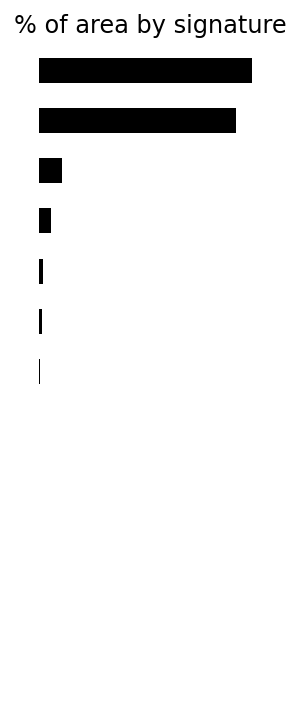
\includegraphics{index_files/figure-pdf/cell-3-output-2.pdf}

}

\end{marginfigure}

The most common class, ``Urban buffer'', is hardly a surprise since the
notion of green belt is worked into its very definition. From the
original signature descriptions\sidenote{\footnotesize \url{https://figshare.com/articles/dataset/Geographical_Characterisation_of_British_Urban_Form_and_Function_using_the_Spatial_Signatures_Framework/16691575/1?file=30935050}},
Urban buffer is:

\begin{quote}
\emph{``Urban buffer'' can be characterised as a green belt around
cities. This signature includes mostly agricultural land in the
immediate adjacency of towns and cities, often including edge
development. It still feels more like countryside than urban, but these
signatures are much smaller compared to other countryside types.}
\end{quote}

However, less than half of green belts are classified as ``Urban
buffer''. The rest is a combination of other classes, including
``Countryside agriculture'' (\textgreater40\%), and ``Open Sprawl''
(\textgreater5\%), as well as a long tail of other signatures with
smaller contributions. To help the reader get a sense of what these
classes represent, we include here the definitions (pen portraits) of
the two most relevant ones:

\begin{itemize}
\tightlist
\item
  Countryside agriculture
\end{itemize}

\begin{quote}
\emph{``Countryside agriculture'' features much of the English
countryside and displays a high degree of agriculture including both
fields and pastures. There are a few buildings scattered across the area
but, for the most part, it is green space.}
\end{quote}

\begin{itemize}
\tightlist
\item
  Open Sprawl
\end{itemize}

\begin{quote}
\emph{``Open sprawl'' represents the transition between countryside and
urbanised land. It is located in the outskirts of cities or around
smaller towns and is typically made up of large open space areas
intertwined with different kinds of human development, from highways to
smaller neighbourhoods.}
\end{quote}

The reader can refer to this additional document for descriptions of all
the classes:

\begin{quote}
\href{https://urbangrammarai.xyz/story/\#ss}{\texttt{https://urbangrammarai.xyz/story/\#ss}}
\end{quote}

\hypertarget{regional-maps}{%
\section{Regional maps}\label{regional-maps}}

The proportions above are national aggregates, and it is possible that
the signature mix varies across different urban areas. To explore this,
below we present maps to explore five English cities.

\hypertarget{london}{%
\subsection{London}\label{london}}

\hypertarget{proportions}{%
\paragraph{Proportions}\label{proportions}}

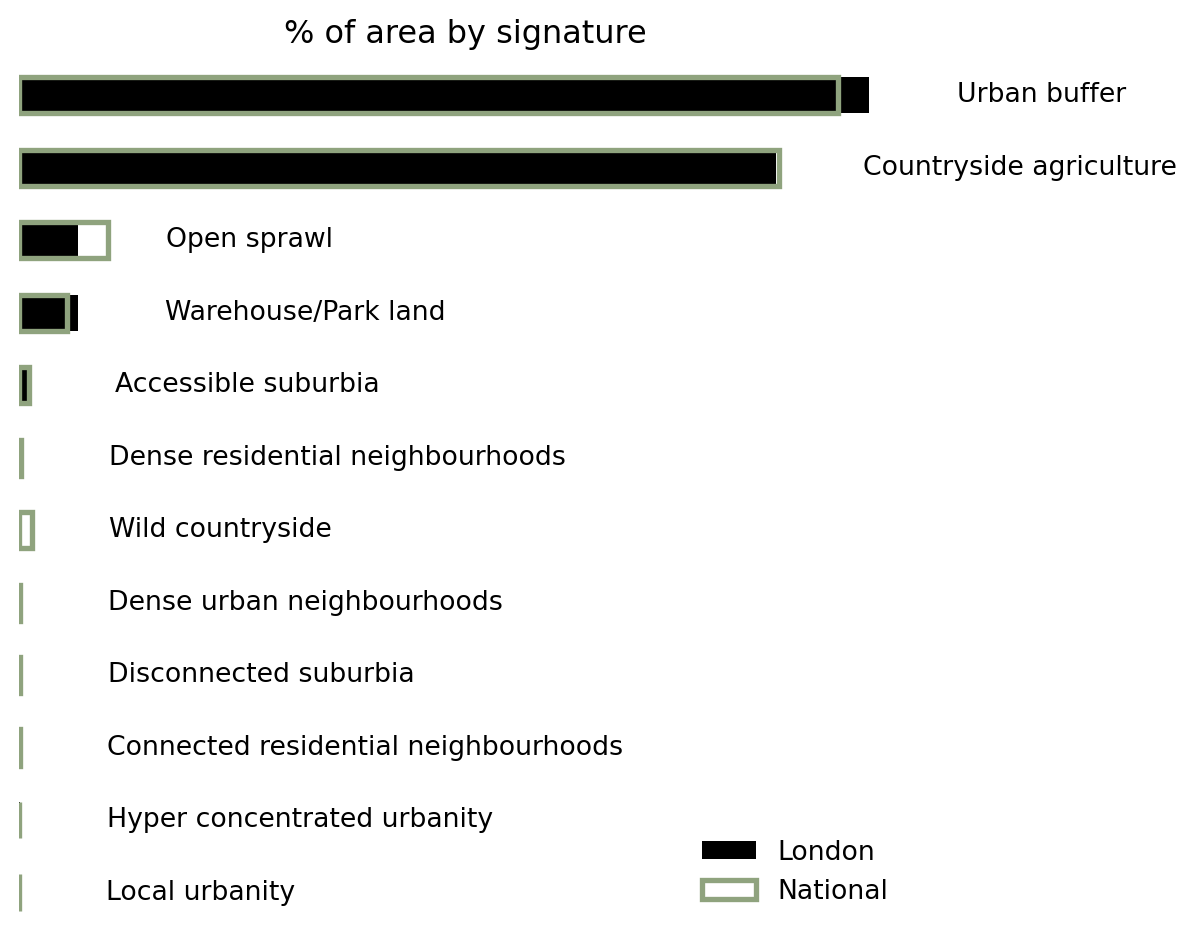
\includegraphics{index_files/figure-pdf/cell-8-output-1.pdf}

\hypertarget{map}{%
\paragraph{Map}\label{map}}

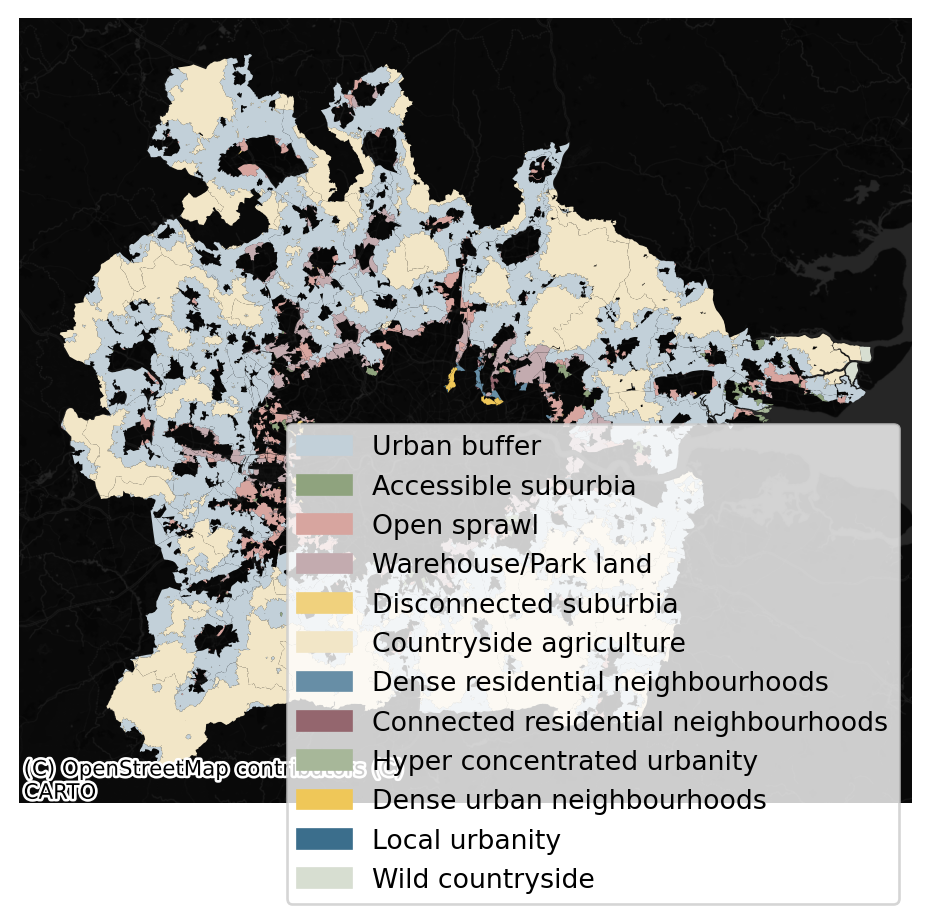
\includegraphics{index_files/figure-pdf/cell-9-output-1.pdf}

\hypertarget{table}{%
\paragraph{Table}\label{table}}

\begin{tabular}{lrr}
\toprule
{} &  Area (Sq.Km) &  \% of total area \\
type                                 &               &                  \\
\midrule
Urban buffer                         &       2499.68 &            48.80 \\
Countryside agriculture              &       2224.66 &            43.44 \\
Open sprawl                          &        173.90 &             3.40 \\
Warehouse/Park land                  &        171.94 &             3.36 \\
Accessible suburbia                  &         24.43 &             0.48 \\
Dense residential neighbourhoods     &          8.06 &             0.16 \\
Wild countryside                     &          7.34 &             0.14 \\
Dense urban neighbourhoods           &          5.39 &             0.11 \\
Disconnected suburbia                &          3.77 &             0.07 \\
Connected residential neighbourhoods &          1.60 &             0.03 \\
Hyper concentrated urbanity          &          0.92 &             0.02 \\
Local urbanity                       &          0.12 &             0.00 \\
\bottomrule
\end{tabular}

\hypertarget{manchester-liverpool}{%
\subsection{Manchester \& Liverpool}\label{manchester-liverpool}}

\hypertarget{proportions-1}{%
\paragraph{Proportions}\label{proportions-1}}

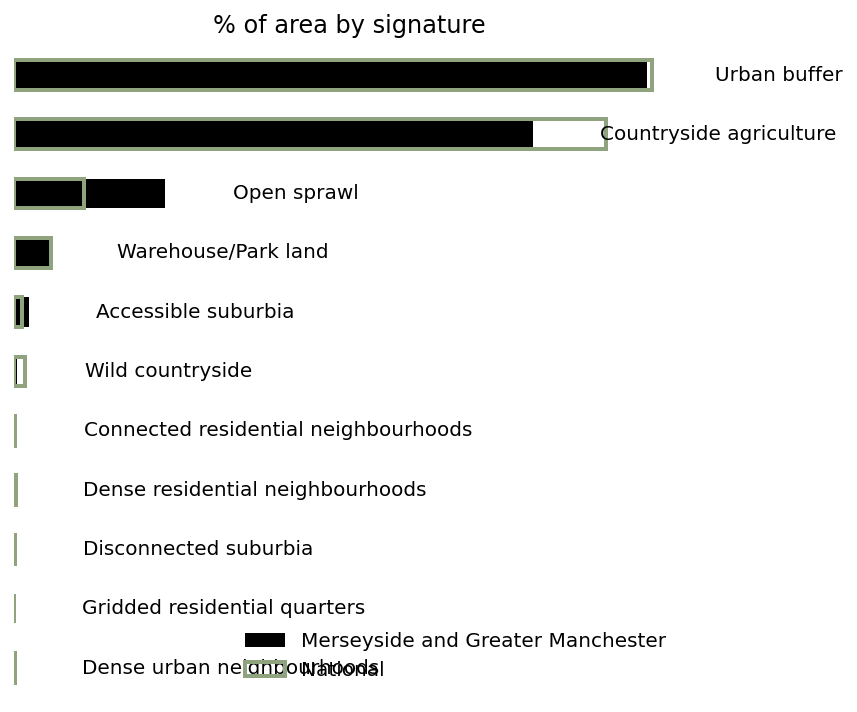
\includegraphics{index_files/figure-pdf/cell-12-output-1.pdf}

\hypertarget{map-1}{%
\paragraph{Map}\label{map-1}}

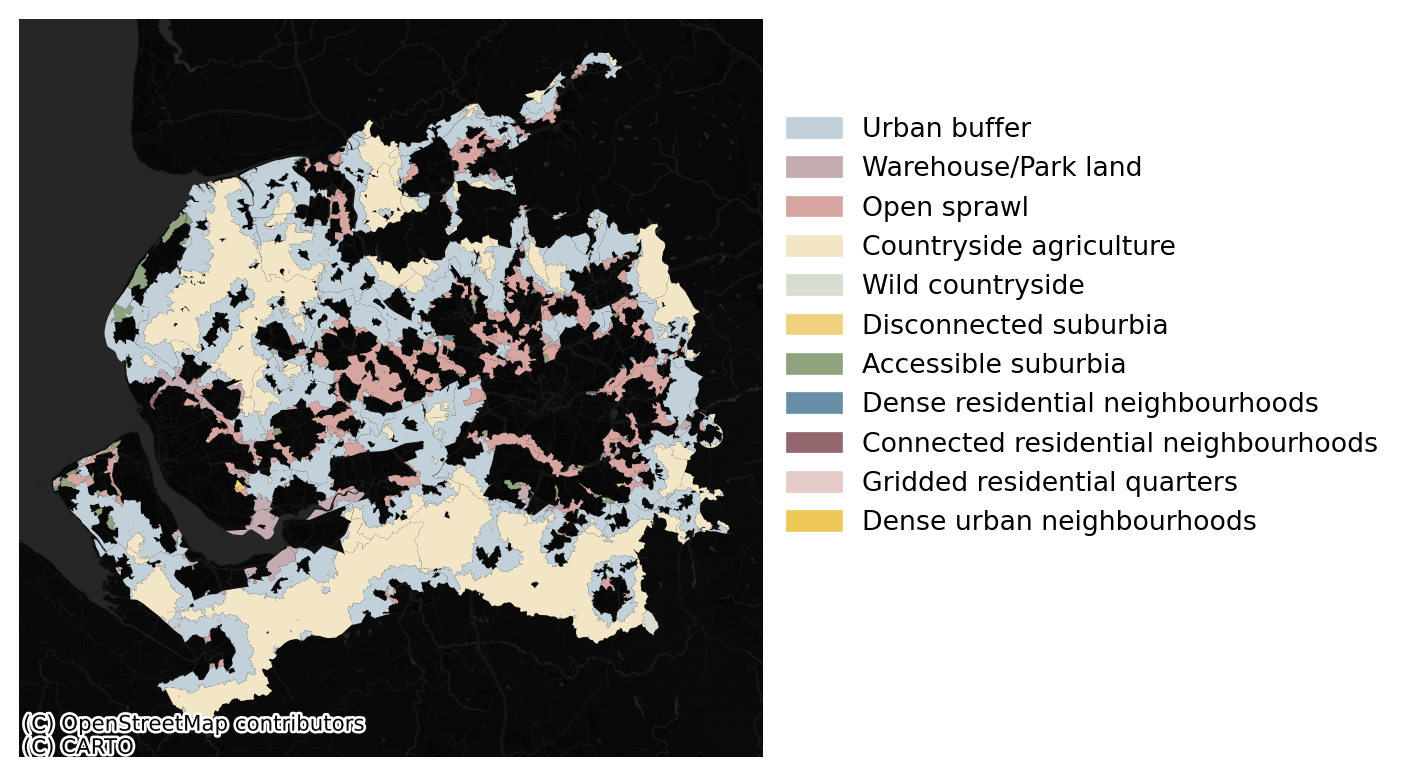
\includegraphics{index_files/figure-pdf/cell-13-output-1.pdf}

\hypertarget{table-1}{%
\paragraph{Table}\label{table-1}}

\begin{tabular}{lrr}
\toprule
{} &  Area (Sq.Km) &  \% of total area \\
type                                 &               &                  \\
\midrule
Urban buffer                         &       1159.74 &            46.63 \\
Countryside agriculture              &        949.70 &            38.19 \\
Open sprawl                          &        276.50 &            11.12 \\
Warehouse/Park land                  &         64.01 &             2.57 \\
Accessible suburbia                  &         26.22 &             1.05 \\
Wild countryside                     &          4.11 &             0.17 \\
Connected residential neighbourhoods &          2.88 &             0.12 \\
Dense residential neighbourhoods     &          2.16 &             0.09 \\
Disconnected suburbia                &          1.52 &             0.06 \\
Dense urban neighbourhoods           &          0.03 &             0.00 \\
Gridded residential quarters         &          0.02 &             0.00 \\
\bottomrule
\end{tabular}

\hypertarget{birmingham}{%
\subsection{Birmingham}\label{birmingham}}

\hypertarget{proportions-2}{%
\paragraph{Proportions}\label{proportions-2}}

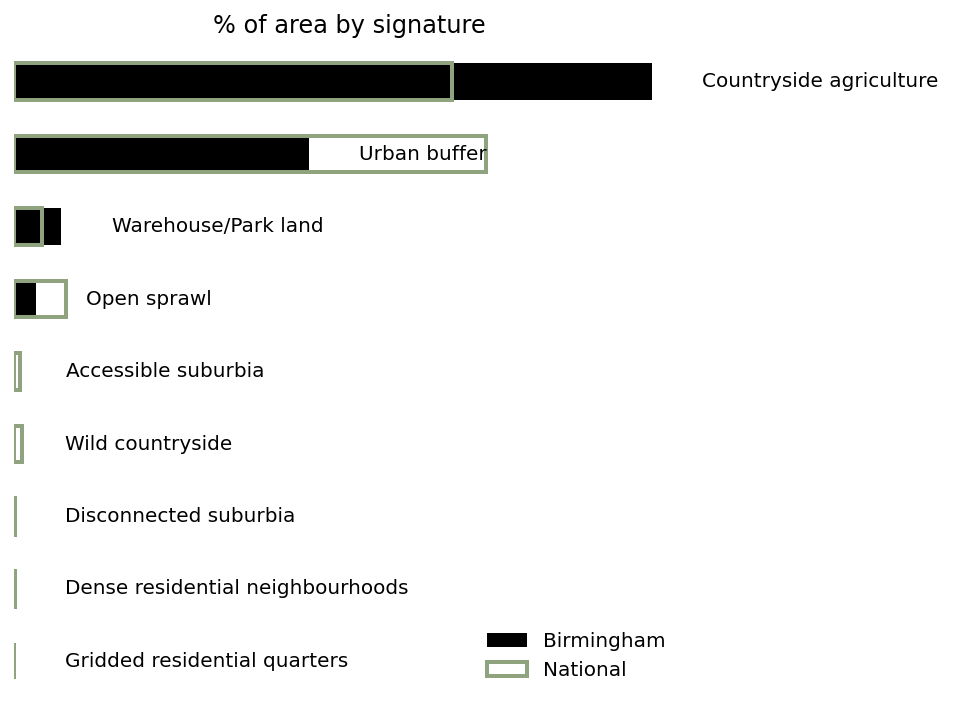
\includegraphics{index_files/figure-pdf/cell-16-output-1.pdf}

\hypertarget{map-2}{%
\paragraph{Map}\label{map-2}}

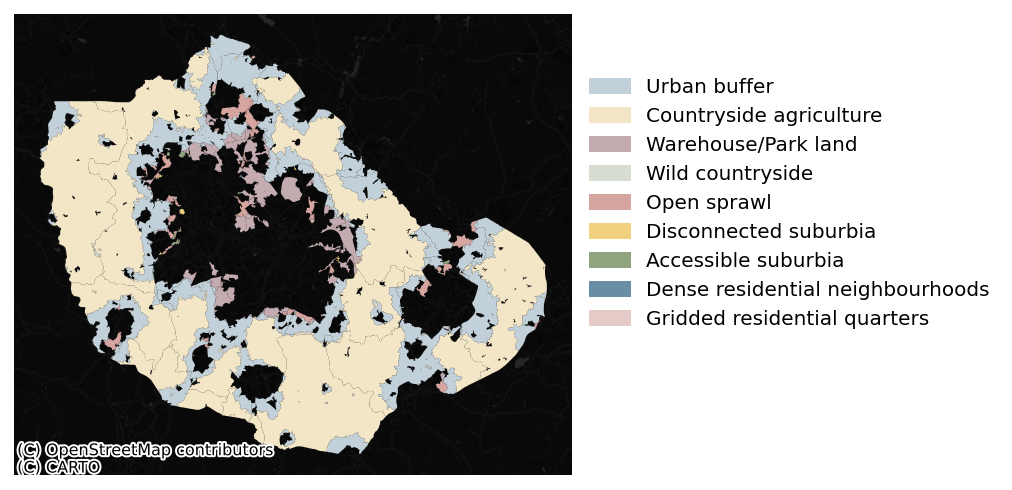
\includegraphics{index_files/figure-pdf/cell-17-output-1.pdf}

\hypertarget{table-2}{%
\paragraph{Table}\label{table-2}}

\begin{tabular}{lrr}
\toprule
{} &  Area (Sq.Km) &  \% of total area \\
type                             &               &                  \\
\midrule
Countryside agriculture          &       1437.69 &            63.59 \\
Urban buffer                     &        663.73 &            29.36 \\
Warehouse/Park land              &        105.94 &             4.69 \\
Open sprawl                      &         48.20 &             2.13 \\
Accessible suburbia              &          2.70 &             0.12 \\
Disconnected suburbia            &          1.19 &             0.05 \\
Wild countryside                 &          1.13 &             0.05 \\
Dense residential neighbourhoods &          0.14 &             0.01 \\
Gridded residential quarters     &          0.06 &             0.00 \\
\bottomrule
\end{tabular}

\hypertarget{newcastle}{%
\subsection{Newcastle}\label{newcastle}}

\hypertarget{proportions-3}{%
\paragraph{Proportions}\label{proportions-3}}

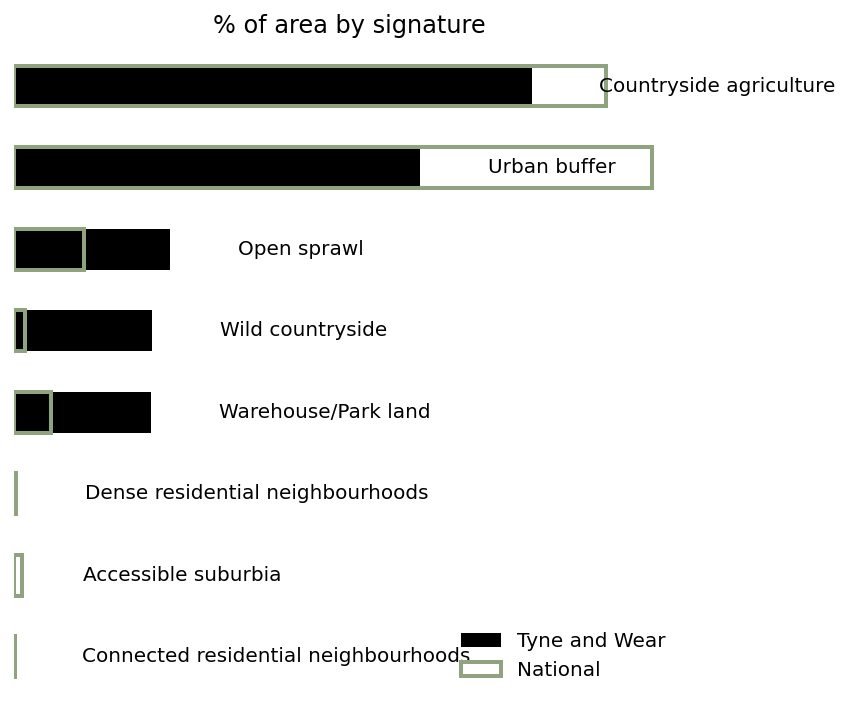
\includegraphics{index_files/figure-pdf/cell-20-output-1.pdf}

\hypertarget{map-3}{%
\paragraph{Map}\label{map-3}}

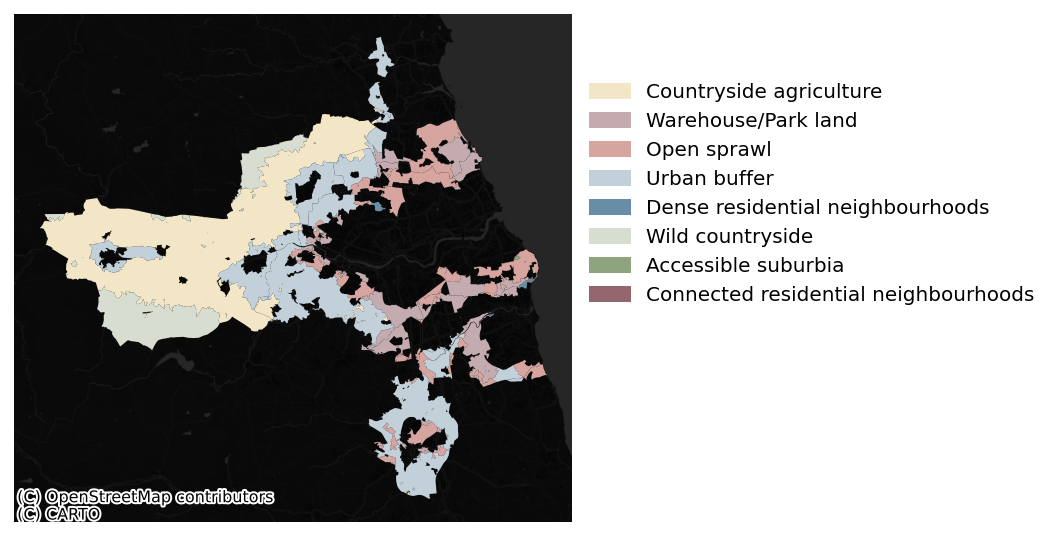
\includegraphics{index_files/figure-pdf/cell-21-output-1.pdf}

\hypertarget{table-3}{%
\paragraph{Table}\label{table-3}}

\begin{tabular}{lrr}
\toprule
{} &  Area (Sq.Km) &  \% of total area \\
type                                 &               &                  \\
\midrule
Countryside agriculture              &        274.99 &            38.12 \\
Urban buffer                         &        215.62 &            29.89 \\
Open sprawl                          &         82.98 &            11.50 \\
Wild countryside                     &         73.17 &            10.14 \\
Warehouse/Park land                  &         72.56 &            10.06 \\
Dense residential neighbourhoods     &          1.72 &             0.24 \\
Accessible suburbia                  &          0.28 &             0.04 \\
Connected residential neighbourhoods &          0.00 &             0.00 \\
\bottomrule
\end{tabular}

\hypertarget{references}{%
\section*{References}\label{references}}
\addcontentsline{toc}{section}{References}




\end{document}
